\chapter{Skizze der Lösungsarchitektur}
\section{Planung und Vorbereitung der Interviews}
Im Rahmen des Projekts werden diverse Interviews durchgeführt, welche ein Schlüsselelement für die Anforderungsanalyse des Projektes bilden.
Diese Methode ermöglicht umfassende Einblicke in die Nutzererfahrungen und Erwartungen an das Planungstool \ac{RAPLA}.
\footcite[Vgl.][567]{baurHandbuchMethodenEmpirischen2014}
Die zeitige Planung für dieses Semester ermöglicht es, frühzeitig wertvolle Erkenntnisse für die Projektentwicklung zu gewinnen und
strategisch in die nächste Phase des Projekts einzusteigen.
\footcite[Vgl.][568]{baurHandbuchMethodenEmpirischen2014}

\section{Entwicklung und Durchführung der Interviews}
Die Entwicklung und Durchführung der Interviews basiert auf einem wohlüberlegten und
strukturierten Ansatz, der die Tiefe und Breite der zu erforschenden Themen vollständig umfasst.
Unser umfangreicher Interviewleitfaden ist sorgfältig ausgearbeitet und orientiert
sich an einem klaren Schema (siehe Abb. \ref{abb:leitfaden}).
\begin{figure}[H]
    \centering
    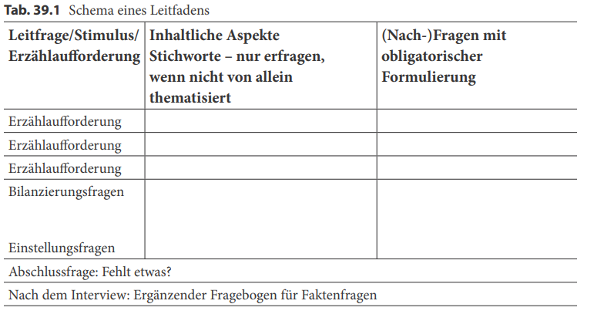
\includegraphics[width=0.9\linewidth]{graphics/leitfaden.png}
    \caption[Schema eines Leitfadens.]{Schema eines Leitfadens.\protect\footnotemark}\label{abb:leitfaden}
\end{figure}
\footnotetext{Enthalten in: \cite{baurHandbuchMethodenEmpirischen2014}, S. 568.}

Jede
Interviewphase ist mit spezifischen Zielen und Fragen verbunden, die darauf abzielen, ein
umfassendes Verständnis von den Erfahrungen der Sekretariatsmitarbeitenden mit digitalen
Werkzeugen sowie ihren Erwartungen an das Planungstool \ac{RAPLA} zu erhalten.

Die Leitfragen dienen als Orientierung für die Befragten, um die Diskussion zu initiieren und sicherzustellen,
dass alle relevanten Themenbereiche abgedeckt sind. Durch die offene Gestaltung wird den Befragten Raum für ihre
persönlichen Berichte und Erfahrungen gegeben. Diese Fragen sind durch inhaltliche Aspekte ergänzt, die als Stichworte dienen und bei
Bedarf abgefragt werden, um sicherzustellen, dass keine wichtigen Informationen ausbleiben.
Diese Stichworte werden nur erfragt, wenn die Teilnehmenden sie nicht von sich aus thematisieren, um die
Natürlichkeit des Gesprächsflusses zu bewahren.
Nachdem die Befragten ihre anfänglichen Gedanken und Erfahrungen geteilt haben, werden Erzählaufforderungen eingeführt,
um tiefere Einblicke und detailliertere Beschreibungen zu erhalten. Diese Aufforderungen helfen, die Erzählung zu
strukturieren und ermöglichen es den Teilnehmenden, ihre Gedanken und Gefühle in Bezug auf das Planungstool RAPLA
detaillierter auszuführen. 

Um ein ausgewogenes Verständnis zu erlangen, werden Bilanzierungsfragen gestellt, die es den Interviewten
ermöglichen, über ihre Erfahrungen zu reflektieren und sie in einen größeren Kontext einzuordnen. Diese Fragen
zielen darauf ab, die Vor- und Nachteile ihrer Erfahrungen mit RAPLA zu bewerten und eine Einschätzung der
Benutzerfreundlichkeit und Funktionalität des Tools vorzunehmen. 
Einstellungsfragen werden genutzt, um die subjektiven Meinungen und Einstellungen der Befragten
zu erfassen. Diese sind entscheidend, um zu verstehen, wie das Tool von den Nutzern wahrgenommen wird
und welche emotionalen und kognitiven Reaktionen es hervorruft. 

Zum Abschluss des Interviews wird die Frage „Für den Fall, dass Ihnen noch ein Aspekt gefehlt hat, welcher wäre dies?“ gestellt,
um es den Teilnehmenden zu ermöglichen,
zusätzliche Gedanken oder Themen einzubringen, die im Laufe des Interviews nicht angesprochen wurden. Dies
dient dazu, sicherzustellen, dass alle relevanten Informationen erfasst werden. 
Durch die Anwendung dieses strukturieren Leitfadens werden konsistente, vergleichbare und aussagekräftige Daten gesammelt.
\footcite[Vgl.][568]{baurHandbuchMethodenEmpirischen2014}
Diese Daten werden letztlich einer sorgfältigen Analyse unterzogen, um eine bestmögliche Anpassung an die Bedürfnisse und Erwartungen
der Nutzer zu gewährleisten.

\section{Integration des Wissensquiz und der Zertifizierung in Moodle}
Die Integration von Wissensbefragung und Zertifizierung in Moodle sind ein kritischer Schritt, um eine umfassende,
zugängliche und nutzerorientierte Bildungserfahrung zu schaffen. Im Zuge der Implementierung wurde sich
für das zweite Arbeitspaket entschieden, welches die Entwicklung und Gestaltung eines Wissensquiz umfasst, welches direkt in
Moodle abgebildet sein wird. Zusätzlich ist eine Zertifizierung zu entwerfen, die den Abschluss des Kurses bestätigt.

Bei der Erstellung des Quiz wird großer Wert darauf gelegt, dass dieses nicht nur informativ, sondern auch
interaktiv und spannend gestaltet wird. Es soll die Nutzer nicht nur testen, sondern auch
Anreize und Motivation zum Lernen bieten. Ferner wird in Betracht gezogen, Elemente der Gamifikation einzuführen.

\section{Gestaltung von Schulungsaufgaben}
Die Schulungsaufgaben werden so gestaltet, dass sie die direkte Anwendung von \ac{RAPLA} in realen Szenarien
widerspiegeln. Hierbei soll zunächst eine Einführung in das Thema mit einer entsprechenden Bearbeitung und Integration
des Nutzers erfolgen. Dadurch soll nicht nur das theoretische Verständnis gefördert werden, sondern es sollen auch praktische
Fertigkeiten geübt und verbessert werden. Darüber hinaus können Fallstudien und realitätsnahe Anwendungsszenarien einbezogen werden,
um die Relevanz und Anwendbarkeit des erlenten Wissens zu stärken.
Die Fragen sollen sowohl thereotische als auch praxisbezogene Übungen beinhalten.
Es wird eine Mischung aus verschiedenen Fragetypen angeboten, um Eintönigkeit zu vermeiden.
\footcite[Vgl.][141]{schweighoferDevelopmentQuizImplementation2019}

Insgesamt zielt die Integration der \ac{RAPLA}-Schulungsaufgaben darauf ab, eine benutzerfreundliche Ugebung zu kreieren,
welche die Nutzer motiviert und schlussendlich dazu befähigt, \ac{RAPLA} effektiv und effizient in ihrem Arbeitsalltag einzusetzen.
\footcite[Vgl.][1]{agambaExploringFacultyIntegration2012}

\section{Bedeutung von Testläufen in der Entwicklung}
Für die Entwicklung von Wissensbefragung und Zertfizierung lassen sich folgende Aspekte in Bezug auf Testläufe festhalten:
\begin{enumerate}
    \item \textbf{Frühe Fehlererkennung und Qualitätsverbesserung:} Die Durchführung von Testläufen während der Entwicklung des Moodle-Quiz ist entscheidend, um frühzeitig Fehler zu erkennen und zu beheben. Diese Vorgehensweise trägt maßgeblich zur Qualitätssteigerung des Endprodukts bei und stellt sicher, dass das Quiz den Lernbedürfnissen der Zielgruppe entspricht.
    \item \textbf{Integration von Probanden in die Konzept- und Entwicklungsphase:} Die Einbeziehung von Testern bereits in der Konzeptphase ermöglicht die Identifikation von Anforderungsdefekten vor ihrer Implementierung. Dies hilft, die Kosten für die Fehlerbehebung zu senken und beschleunigt den Entwicklungsprozess, indem ein tiefgehendes Verständnis für das Projekt entwickelt wird.
    \item \textbf{Sicherstellung der Softwarezuverlässigkeit:} Durch Pilot-Tests mit einer ausgewählten Nutzergruppe wird wertvolles Feedback gesammelt, das für die Anpassung des Quiz entscheidend ist. Diese Tests gewährleisten die Sicherheit und Zuverlässigkeit des Moodle-Quiz, indem sie sicherstellen, dass es in realen Szenarien sicher verwendet werden kann, was für die Zielgruppe von entscheidender Bedeutung ist.
\end{enumerate}
Durch diese strukturierte Einbindung von Testläufen in den Entwicklungsprozess wird sichergestellt, dass das Moodle-Quiz nicht nur fehlerfrei, sondern
auch optimal auf die Bedürfnisse und Präferenzen der Nutzer zugeschnitten ist.